\chapter{Image Style Transfer}\chlbl{image_style_transfer}
In the field of image style transfer\sidecite{Gatys_Ecker_Bethge_2015}, such correlations are used to generate images.
An image is created based on two images, one image providing the content (i.e. the ``content-image'') and the other image providing the style (i.e. the ``style-image'').
To generate the content of the image, a random image can be fed into the model and a simple distance-based loss function such as the Euclidean norm can be used to calculate the difference between the model output and the content-image.
Over time, the model would learn to output the content-image.
However, only the content from the content-image and not its style is needed.
A solution to this problem is using Convolutional feature maps\sidenote{a convolutional layer can have multiple filters (i.e. channels), each filter produces a convolutional feature map} as they capture spatial information of an image well, while containing only little style information.
Therefore, the distance loss is not calculated between the content-image and the model output but between the feature maps of the content-image and the output image.

The second task is to transfer the style from the style-image to the model output.
The style of an image can be described by correlations across the different feature maps.
This information about the image style can be calculated with a Gram matrix.
A Gram matrix is the dot product\sidenote{the dot product between two vectors can be seen as similarity metric; it gets bigger if two vectors are more similar} of the flattened feature vectors from a convolutional feature map (i.e. the dot product between all channels of a convolutional layer's output).
For example, a convolutional layer could have multiple channels. The first channel could have a high activation for black and white stripes in horizontal direction while the second channel could have a high activation for black and white stripes in vertical direction. If both channels activate together for the same input and thus have a high correlation, there is a high possibility that the image might contain the style of a chessboard (i.e. black and white checkered). A third channel, for example, could have a high activation for eyes. If this channel has a low correlation with the first channel but a high correlation with the second channel (i.e. black and white stripes in vertical direction), the input image might contain the face of a zebra and thus capture a ``zebra-style''.
Similar to the content-transfer, a distance loss such as the Euclidean distance can be used to compare the Gram matrices of the style-image and the output-image.
Thus, it is compared if the output-image has the same style as the style-image.

In summary, the content is transferred by comparing entire convolutional layer output and the style by comparing the correlations between the feature maps of a convolutional layer output (i.e. by comparing gram matrices).

%\pagebreak
%\chapter{Design Decisions}\chlbl{design_decisions}
%There exists a variety of possibilities how self-organization of the network architecture can be implemented.
%However, this thesis is of course limited in time and resources an thus not all of them can be investigated.
%Therefore, a promising direction of research had to be defined at the beginning and followed afterwards.

%As a constraint it was defined that (i) a network without dynamics is developed and (ii) self-organization takes place across multiple layers.
%A network without dynamics is used because Deep Learning works very well for pattern recognition and the data analyzed by the computer is mostly static.
%Dynamic networks usually have poorer performance and use special algorithms to convert static data such as images into dynamic time-related signals (c.f. Section \secref{self_org_spiking}).
%Applying self-organization across multiple layers rather than just adding lateral connections in one layer is preferred as this allows the network to form more complex structures and thus to use the whole potential of self-organisation.

%This thesis is strongly inspired by the paper ``Natural Intelligence'' \sidecite{von_der_Malsburg_Stadelmann_Grewe_2022} (c.f. Section \secref{natural_intelligence}).
%The most relevant findings in this work are:

%\begin{itemize}
%  \item The brain is highly structured
%  \item Self-organization is the most promising approach to achieve natural intelligence. It loops between activity and connectivity
%  \item Self-organization forms net-fragments, one neuron can be part of multiple fragments
%  \begin{itemize}
%    \item An object can be represented by multiple net-fragments
%    \item A hierarchy of features can be represented by nested net-fragments
%  \end{itemize}
%  \item The self-organizing process has to start from an already established coarse structure
%  \item There exists many alternative pathways in the network
%\end{itemize}

%However, it is unclear how these findings and hypotheses from the field of neuroscience can be implemented in an algorithm.
%To create a self-organizing neural network, the following mechanisms are particularly relevant: The design of the initial architecture, the allowed architecture modifications (removing and adding neurons and/or connections), the type of neurons, and the definition of the learning algorithm.
%These aspects are discussed hereafter.

%\begin{description}
%   \item[Design of initial architecture] The initial architecture should exhibit a good inductive bias from the start so that the network can learn (something meaningful). Current approaches also start from much bigger architectures and reduce their size by up to a thirty-fold \sidecite{Pedersen_Risi_2021} (c.f. Section \secref{self_org_related}) or grow the architecture from a single neuron \sidecite{Raghavan2019NeuralNG} (c.f. Section \secref{self_org_spiking}) by using self-organisation.
%   \item[Architecture modifications] The architecture can be modified in several ways. For example, from a more global perspective, the network can grow, shrink, split into sub-networks\sidenote{this is related to ensemble approaches TODO: add source}, or multiple sub-networks can re-organize into one network. From a local perspective, connections can be created or removed within the same layer (lateral connections) or between subsequent layer. Moreover, connections can be used to skip on or several layers (residual connections), or connections can be recurrent to a previous layer. Furthermore, besides modifying single connections and neurons, complete blocks of neurons can be added or removed. This includes for example layers, mathematical functions like pooling operations, or pre-defined modules consisting of several layers.
%   \item[Type of neurons] As described above, no dynamic (i.e. spiking) neurons are employed. The classical neurons multiply the input \(\boldsymbol{x}\) by a weight vector \(\boldsymbol{w}\), add a bias \(\boldsymbol{b}\) and calculate the output with a non-linear activation of this sum (c.f. Section \secref{ann}). However, recent architectures replace such classical neurons with more complex units. For example, Kirsch and Schmidhuber \sidecite{kirsch2021meta} (c.f. Section \secref{self_org_related}) use tiny RNNs with shared parameters as neurons. Such neurons are able to learn learning algorithms which are equivalent to back-propagation.
%   \item[Learning algorithm] ... (see learning to learn or Hebbian based on input covarinace or learning based on target label (e.g. enforce some distinction in neurons covariance matrix depending on label))
%\end{description}


\chapter{Experiments Hebbian Learning}\chlbl{exp_hebb_learning}
I used different variants of Hebbian Learning with the goal of generating good latent representations of visual scenes.
However, all preliminary experiments with different implementations were not promising.
In my experiments, classical Hebbian learning (as described in Equation \eqref{hebb_1}) led to symmetric weights, which in turn led to poor representations.
This symmetry could be broken by using the ABCD-Hebbian learning rule \sidecite{Niv_Joel_Meilijson_Ruppin_2001}.
The ABCD learning rule calculates the weight update \(\Delta w_{ij}\) from neuron \(i\) to neuron \(j\) based on the pre-synaptic activity \(r_i\) of neuron \(i\) and post-synaptic activity \(r_j\) of neuron \(j\) as follows:

\begin{equation}\eqlbl{hebb_abcd}
	\Delta w_{ij} = \eta_w \cdot (A_wr_ir_j+B_wr_i+C_wr_j+D_w)
\end{equation}

where \(\eta_w\) is a weight-specific learning rate, and \(A_w\) is a correlation coefficient, \(B_w\) is a presynaptic coefficient, \(C_w\) is a postsynaptic coefficient, and \(D_w\) is a bias coefficient.
The bias coefficient \(D_w\) can be interpreted as an individual inhibitory or excitatory bias of each connection in the network.
Similar to Najarro and Risi \sidecite{NEURIPS2020_ee23e7ad}, the coefficient were learnt through an evolution strategy \sidecite{Salimans_Ho_Chen_Sidor_Sutskever_2017}.
However, this method does not scale for large networks with many parameters and did not achieve the desired performance in my experiments.

Of course, it cannot be concluded from these experiments that Hebbian Learning cannot be used to learn networks for extracting good representation from visual scenes.
However, it was found that it is not trivial and that just applying the Hebbian learning rule is not sufficient, especially if the network has a structure of modern Deep Learning architectures with many parameters.

However, in further preliminary experiments it was found that Hebbian Learning has interesting properties for pruning.
A good performing CNN was created and trained on MNIST with backpropagation.
The network consists of two convolutional layers, followed by a pooling layer and three linear layers.
The first convolutional layer increases the number of channels from \([\text{width} \times \text{height} \times \text{n\_channels}]\) to \([\text{width} \times \text{height} \times 32]\).
The second convolutional layer further increases the number of channels to \([\text{width} \times \text{height} \times 64]\).
The subsequent max. pooling layer decreases the size to \([\text{width}/2 \times \text{height}/2 \times 64]\).
The activation map is then flatten and fed into 3 fully connected layers with an output size of \(1024\), \(128\), and \(10\) respectively.
Between each layer, ReLU activtions are employed.
The network is visualized in Figure \figref{hebb_pruning}.

\begin{figure}[h]
    \centering
    \resizebox{0.99\textwidth}{!}
{
	\begin{tikzpicture}
		\tikzstyle{connection}=[ultra thick,every node/.style={sloped,allow upside down},draw=\edgecolor,opacity=0.7]
\tikzstyle{copyconnection}=[ultra thick,every node/.style={sloped,allow upside down},draw={rgb:blue,4;red,1;green,1;black,3},opacity=0.7]


\pic[shift={(0,0,0)}] at (0,0,0) 
    {Box={
        name=conv1,
        caption=Conv + ReLU,
        xlabel={{1, }},
        zlabel=32,
        fill=\ConvColor,
        height=16,
        width=4,
        depth=16
        }
    };


\pic[shift={(3,0,0)}] at (0,0,0) 
    {Box={
        name=conv2,
        caption=Conv + ReLU,
        xlabel={{32, }},
        zlabel=64,
        fill=\ConvColor,
        height=16,
        width=8,
        depth=16
        }
    };


\draw [connection]  (conv1-east)    -- node {\midarrow} (conv2-west);


\pic[shift={ (0,0,0) }] at (conv2-east) 
    {Box={
        name=pool1,
        caption= ,
        fill=\PoolColor,
        opacity=0.5,
        height=8,
        width=1,
        depth=8
        }
    };


\pic[shift={(4,0,0)}] at (pool1-east) 
    {Box={
        name=fcn1,
        caption=Hebb. Pruning + ReLU,
        xlabel={{" ","dummy"}},
        zlabel=1024,
        fill=\SoftmaxColor,
        opacity=0.8,
        height=3,
        width=3,
        depth=100
        }
    };


\draw [connection]  (pool1-east)    -- node {\midarrow} (fcn1-west);


\pic[shift={(2,0,0)}] at (fcn1-east) 
    {Box={
        name=fcn2,
        caption=Hebb. Pruning + ReLU,
        xlabel={{" ","dummy"}},
        zlabel=128,
        fill=\SoftmaxColor,
        opacity=0.8,
        height=3,
        width=3,
        depth=50
        }
    };


\draw [connection]  (fcn1-east)    -- node {\midarrow} (fcn2-west);


\pic[shift={(2,0,0)}] at (fcn2-east) 
    {Box={
        name=fcn3,
        caption=FCN + Softmax,
        xlabel={{" ","dummy"}},
        zlabel=10,
        fill=\SoftmaxColor,
        opacity=0.8,
        height=3,
        width=3,
        depth=25
        }
    };


\draw [connection]  (fcn2-east)    -- node {\midarrow} (fcn3-west);

\end{tikzpicture}
}
    \caption[Hebbian Pruning Network]{The network architecture used to perform Hebbian-based weight pruning.}
    \figlbl{hebb_pruning}
\end{figure}

The image classification model is trained with backpropagation to minimize the negative log likelihood (NLL) loss.
Adam \sidecite{Kingma_Ba_2017} is used as optimization algorithm with a mini-batch size of \(32\) a learning rate of \(5\cdot 10^{-4}\).
As soon as the loss reaches a plateau, the learning rate is reduced to \(1\cdot 10^{-4}\).

After the model is trained, the first two fully connected layers within the network are pruned with Hebbian learning based methods.
The convolutional layers cannot be pruned because such layers employ a convolutional function that impedes calculating the correlation between an input and an output neuron.
The last layer, on the other hand, cannot be pruned as it corresponds to the number of classes.

The \emph{first} Hebbian based method proposed pushes the weights between neuron \(i\) and neuron \(j\) towards \(0\) if \(i\) and \(j\) have a low correlation within a mini-batch.
First, a mini-batch is sampled.
Afterwards, the correlation between \(i\) and \(j\) is calculated for each sample.
if the correlation is below \(0.02\) for at least \(20\%\) of the samples (i.e. \(7\) samples or more for a mini-batch size of \(32\)), the weight is updated as follows:
\begin{equation}\eqlbl{hebb_towards_0}
	\Delta w_{ij} = - \eta_H \cdot w_{ij}
\end{equation}

where \(\eta_H\) is the Hebbian learning rate set to \(1\cdot 10^{-5}\).

The \emph{second} Hebbian based method proposed pushes some of the weights exactly to \(0\) while all other weights remain the same.
During an epoch, the correlation between neurons \(i\) and \(j\) is measured for each weight \(w_{ij}\).
Afterwards, the weights with the lowest correlations are set to \(0\).
How many weights are set to \(0\) is a hyper-parameter that has to be specified in advance.

For both methods, the model is pre-trained and pruned on the MNIST dataset \cite{MNIST} and evaluated on the MNIST as well as on the MNIST-C\sidenote{MNIST-C is a corrupted version of MNIST and well suited to measure model robustness} dataset \cite{Mu_Gilmer_2019}.
The \emph{first} Hebbian based method can improve the results even after backpropagation as shown in Table \tabref{nll_hebb_pruning}.

\begin{table}[h] 
    \tablbl{nll_hebb_pruning}
    \centering
	 \begin{tabular}{|l c c|} 
    	\hline
    	 & NLL-Loss & NLL-Loss \\
        Dataset & without Hebbian Updates & with Hebbian Updates\\
        \hline
        MNIST & \(0.05314\) & \(0.03386\) \\
        MNIST-C & \(0.6013\) & \(0.4766\) \\
        \hline
    	 &Accuracy & Accuracy \\
        Dataset & without Hebbian Updates & with Hebbian Updates\\
        \hline
        MNIST & \(98.94\%\) & \(98.97\%\) \\
        MNIST-C & \(88.74\%\) & \(89.94\%\) \\
        \hline
    \end{tabular}
    \caption[NLL Loss of Hebbian Pruning Network]{NLL loss of the model before and after the \emph{first} Hebbian-based pruning method.}
\end{table}

The NLL-loss on the MNIST test dataset decreases from \(0.05314\) to \(0.03386\), while the loss on MNIST-C test dataset decreases from \(0.6013\) to \(0.4766\) after applying the \emph{first} Hebbian based method.
However, in terms of accuracy the improvements are marginal.
Furthermore, it has to be considered that this is only a preliminary experiment and this method certainly offers various potential for improvement.
This experiments indicates that Hebbian in combination with back-propagation could lead to better or more robust representations because the Hebbian updates improved performance on both datasets.

The \emph{second} Hebbian based method sets weights between neurons with a low correlation to \(0\).
The network trained with back-propagation has an accuracy of \(98.94\%\) on MNIST.
By setting up to \(40\%\) of the weights to \(0\), the accuracy remains above \(>98\%\).
Setting weights to \(0\) can make the network smaller and more efficient \sidecite{Liang_Glossner_Wang_Shi_Zhang_2021}.
Furthermore, it leads to sparse representations that can improve robustness.
Figure \figref{hebb_prune} visualizes the loss of the \emph{second} Hebbian based method for different ratios of kept weights.
Furthermore, the correlation based method is compared to randomly setting the same fraction of weights to \(0\).

\begin{figure}[h]
    \centering
    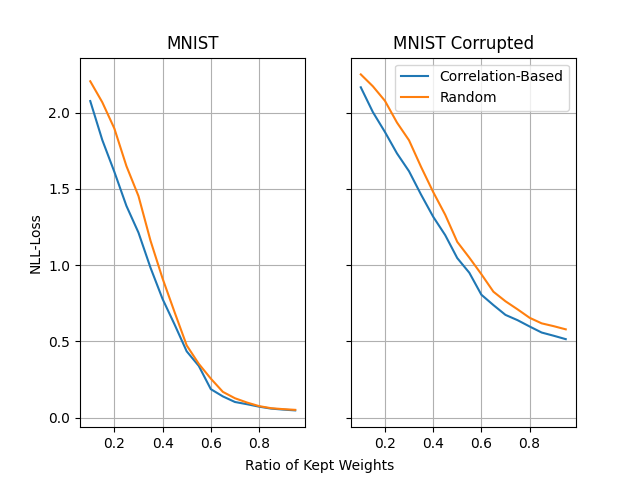
\includegraphics[width=0.99\textwidth]{loss_hebb_pruning}
    \caption[NLL Loss of Hebbian Pruning]{The NLL loss of the \emph{second} Hebbian based pruning method compared to removing random weights. The y axis shows the loss while the x axis shos the ratio of weights kept. }
    \figlbl{hebb_prune}
\end{figure}

It can be observed that the performance is better when weights between neurons with low correlation are set to \(0\) than if random weights are set to \(0\).


